\documentclass[sigconf, nonacm, onecolumn]{acmart}

\usepackage[utf8]{inputenc}
\usepackage[T1]{fontenc}
\usepackage{lmodern}
\usepackage{graphicx}
\usepackage{booktabs}
\usepackage{amsfonts}
\usepackage{amsmath}
\usepackage{nicefrac}

%% ----------------------------------------------------------------
%% Title
%% ----------------------------------------------------------------
\title{Mitigating Reasoning Hallucinations in LLMs via
Neuro-Symbolic Integration for Ill-Defined
Mathematical Problems}

%% ----------------------------------------------------------------
%% Authors
%% ----------------------------------------------------------------
\author{Jave Bacsain}
\affiliation{%
  \department{College of Computer Studies}
  \institution{Camarines Sur Polytechnic Colleges}
  \country{Philippines}
}
\email{javbacsain@my.cspc.edu.ph}

\author{Ivy Pauline Muit}
\affiliation{%
  \department{College of Computer Studies}
  \institution{Camarines Sur Polytechnic Colleges}
  \country{Philippines}
}
\email{ivmuit@my.cspc.edu.ph}

%% ----------------------------------------------------------------
\begin{document}

\begin{teaserfigure}
  \centering
  
\includegraphics[width=3cm]{logo.png}\\[4pt]
  {\small CSAC 224 -- Natural Language Processing}
\end{teaserfigure}

\maketitle

%% ----------------------------------------------------------------
\section{Abstract}

Large Language Models (LLMs) frequently produce confident yet incorrect
answers to mathematical problems that are missing key information or contain
contradictory conditions. We implement and evaluate a hybrid neuro-symbolic
pipeline in which a few-shot prompted language model translates a math word
problem into SMT-LIB v2 and the Z3 constraint solver makes the final decision:
a unique satisfying model yields the numeric answer, \texttt{UNSAT} signals a
contradiction, and multiple satisfying models signal missing information. On a
balanced 600-problem test set drawn from the PMC benchmark (ill-defined
problems) and GSM8K (solvable problems), the pipeline using
Qwen2.5-7B-Instruct reduces the rate of confident wrong answers on ill-defined
problems from 19--21\% to 2\%, a roughly ten-fold reduction, and is the only
system that explicitly detects any contradictions. When evaluation is framed
as a binary reject-vs-solve decision, the pipeline's F1 on the rejection
class (0.799) is within 9\% of the best baseline (0.880). The trade-off is
that the 7B translator under-constrains its SMT-LIB output on roughly 80\%
of solvable inputs, causing the pipeline to over-abstain and trail the
baselines on three-class macro F1 (0.210 vs.\ 0.474--0.482). The results
support the project's hypothesis that separating language understanding from
logical evaluation eliminates a class of hallucinations unreachable by
prompted LLMs, while indicating that closing the macro-F1 gap requires either
a fine-tuned translator or a larger base model.

%% ----------------------------------------------------------------
\section{Introduction}

Modern Large Language Models (LLMs), systems trained to predict the next word
in a sequence, have become surprisingly capable at answering questions in
plain language~\cite{brown2020}. However, they have a structural weakness:
because they are trained to produce \textit{plausible} text, they often
generate a confident-sounding answer even when no correct answer
exists~\cite{huang2025}. This tendency is known as hallucination.

The problem is especially damaging in mathematics. Real-world applications in
fields such as finance, healthcare, and engineering frequently involve
problems with missing data or conflicting requirements~\cite{puchalska1987}. A
student who forgets to include a key value in their homework, or a dataset
with an entry error, can produce a problem that is mathematically unsolvable,
yet standard LLMs will still produce a numeric answer with apparent
confidence.

The input to our algorithm is a math word problem written in plain English.
The output is either (i) a numeric answer if the problem is solvable, or (ii)
a \texttt{REJECT} label if the problem is ill-defined (missing information or
contradictory constraints). The system uses a language model not to solve the
problem directly, but to describe the problem's logical structure in a format
that an external constraint solver can evaluate rigorously. This separation
prevents the model from fabricating answers at the reasoning stage. Our main
contribution is an empirical study of this design on the PMC
benchmark~\cite{zhou2024} that quantifies the trade-off between aggregate
accuracy and hallucination rate on ill-defined inputs.

This project is being submitted exclusively for this Natural Language
Processing class, and its components have not been used for any other courses.

%% ----------------------------------------------------------------
\section{Related Work}

Prior work on improving the reasoning ability of language models can be
grouped into three categories: prompting strategies, tool-assisted approaches,
and logic-based systems.

\textbf{Prompting Strategies.} Chain-of-Thought (CoT)
prompting~\cite{wei2022} improved language model reasoning by asking the
model to write out intermediate steps before giving a final answer. Kojima et
al.~\cite{kojima2022} extended this by showing that the single fixed phrase
``Let's think step by step'' can trigger the same behavior without
task-specific examples. Program of Thoughts (PoT)~\cite{chen2023} goes
further by having the model write a small Python program instead of natural
language steps, letting a code interpreter handle the arithmetic.
MathPrompter~\cite{imani2023} generates multiple independent solutions to the
same problem and checks whether they agree before committing to an answer.
Lightman et al.~\cite{lightman2024} showed that providing feedback on each
individual reasoning step during training, rather than only on the final
answer, significantly reduces logical errors in multi-step problems.
Self-Consistency~\cite{wang2023sc} also marginalizes over multiple sampled
reasoning paths to improve reliability. None of these approaches addresses
the case where a problem has no valid solution; the model will still attempt
to produce one.

\textbf{Tool-Assisted Language Models.} A second line of work connects
language models to external tools. Program-Aided Language Models
(PAL)~\cite{gao2023} delegate arithmetic steps to a Python interpreter. The
Chameleon framework~\cite{lu2023} treats the language model as a planner
that decides which external tool to call. ReAct~\cite{yao2023} interleaves
reasoning steps with real-world actions such as looking up facts.
Toolformer~\cite{schick2023} demonstrated that a language model can be
trained to decide on its own when to call an external tool. While these
systems extend what a language model can do, they are oriented toward
finding an answer, not toward recognizing when an answer cannot exist.

\textbf{Formal Logic and Neuro-Symbolic Systems.} The closest work to this
project involves converting natural language problems into formal logical
representations and using dedicated solvers to evaluate them.
Logic-LM~\cite{pan2023} uses a language model to translate a problem into a
symbolic logic format which is then evaluated by an external logic engine.
SATLM~\cite{ye2023} takes a similar approach, framing problems as
satisfiability queries and passing them to the Z3 constraint
solver~\cite{demoura2008} to determine whether a valid solution exists. Both
systems outperform purely generative approaches on structured reasoning
tasks. A specialized study~\cite{heyueya2023} combined language models with
an external symbolic solver (SymPy, an algebraic system) for math word
problems, showing that delegating computation to a deterministic solver
reduces errors significantly. NS-CL~\cite{mao2019} demonstrated similar
neuro-symbolic gains in visual reasoning by combining a learned visual
parser with a deterministic symbolic executor. Most directly related to this
work, VCSearch~\cite{zhou2024} is a concurrent training-free framework that
uses formal language to detect ill-defined problems on the PMC benchmark via
a variable-constraint search strategy.

This project extends the above line of work in two ways. First, while
Logic-LM, SATLM, and related systems assume that every problem has a valid
answer and focus on finding it, our system specifically targets ill-defined
problems and is evaluated on its ability to correctly
abstain~\cite{puchalska1987,zhou2024}. Second, unlike VCSearch's
variable-constraint search strategy, we use a \emph{few-shot prompted}
translator paired with an SMT solver and distinguish Missing-type
(infinitely many satisfying models) from Contra-type (UNSAT) cases through
solver semantics directly. This shifts the goal from ``solve the problem''
to ``determine whether the problem can be solved.''

%% ----------------------------------------------------------------
\section{Data \& Resources}

\subsection{Test Set Construction}

We evaluate on a balanced 600-problem test set built from two public
sources:

\begin{itemize}
  \item \textbf{PMC}~\cite{zhou2024} (Hugging Face dataset
  \texttt{kevin715/PMC}). PMC is a test-only benchmark of ill-defined
  mathematical word problems built by seeding from four well-defined math
  benchmarks (GSM8K, SVAMP, AddSub, MultiArith) and introducing either
  missing information or a contradictory constraint, with each ill-defined
  variant validated by both LLMs and human annotators. We sample 200
  problems from its \texttt{missing\_test} split (3{,}285 problems
  available) and 200 from its \texttt{contra\_test} split (2{,}088
  available).
  \item \textbf{GSM8K}~\cite{cobbe2021} (Hugging Face dataset
  \texttt{openai/gsm8k}, \texttt{main} config). GSM8K is a widely-used
  benchmark of grade-school arithmetic word problems with verified integer
  answers. We sample 200 problems from its \texttt{test} split (1{,}319
  available).
\end{itemize}

Each row of the resulting \texttt{test.jsonl} has the schema
\texttt{\{id, problem, label, answer\}} where \texttt{label} is one of
\texttt{solvable}, \texttt{missing}, or \texttt{contra}, and
\texttt{answer} is an integer (for solvable rows) or \texttt{null}
otherwise. Sampling uses a fixed random seed (42) for reproducibility.

\subsection{Preprocessing}

We feed each problem text to the model without modification beyond the
model's own sub-word tokenization. Out-of-vocabulary mathematical symbols
are handled by the BPE tokenizer of the chosen base model. We do not
normalize numerals or unit strings; this is by design, so that the
translation step (Section~\ref{sec:method}) is forced to handle real-world
problem text rather than a pre-cleaned subset.

\subsection{Seed Examples for Few-Shot Prompting}

We hand-crafted 10 (problem, SMT-LIB) demonstration pairs covering the three
classes (three solvable, three contradictory, four missing-information).
Each demonstration was independently verified by running its SMT-LIB through
Z3 and checking that the solver's verdict matched the intended class. The
seed file is included with the project's source code release.

\subsection{Departures from the Midterm Proposal}

The midterm proposal assumed PMC would be split into 4{,}000 training /
500 validation / 500 test rows and that the translator would be
fine-tuned with LoRA~\cite{hu2022} on auto-generated SMT-LIB labels. After
inspecting the released PMC dataset, we found that PMC is test-only (no
training split, no answer field for ill-defined rows). The proposal also
treated PMC's source as exclusively GSM8K, but PMC is seeded from four
benchmarks. We therefore restructured the experimental setup to: (i) drop
the fine-tuning step in favor of a few-shot prompted translator, and (ii)
introduce GSM8K test-split problems as the solvable class. This change is
discussed further in Section~\ref{sec:method}.

%% ----------------------------------------------------------------
\section{Methodology}
\label{sec:method}

\subsection{Pipeline Overview}

The system consists of two components running in sequence: a few-shot
prompted language model that reads a math problem and produces a formal
logical description, and an external constraint solver that evaluates that
description. Figure~\ref{fig:pipeline} summarizes the pipeline.

\begin{figure}[htbp]
  \centering
  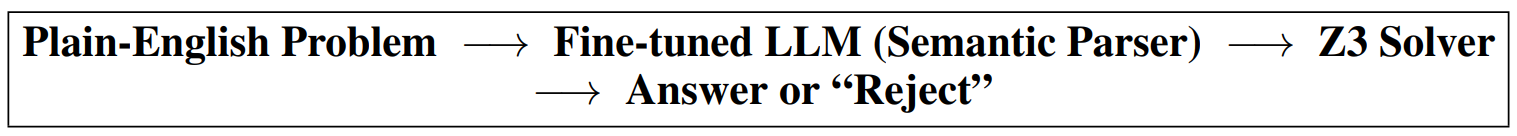
\includegraphics[width=0.85\columnwidth]{pipeline.png}
  \caption{Overview of the two-stage neuro-symbolic pipeline.}
  \label{fig:pipeline}
\end{figure}

\subsection{Stage 1: Language Model as a Translator}

The language model's role is not to solve the math problem but to translate
a problem into SMT-LIB v2~\cite{barrett2010}, a standardized text format
used to describe logical constraints (analogous to how a programming
language describes instructions for a computer). The system prompt
instructs the model to: (i) declare each unknown with
\texttt{(declare-const <name> Int|Real)}; (ii) encode every stated
constraint as an \texttt{(assert ...)}; (iii) add
\texttt{(assert (>= <name> 0))} for any natural quantity (counts, money,
distance, time), since real-world quantities cannot be negative and this
implicit constraint is needed for Z3 to detect contradictions such as
``subtract more than you have''; (iv) terminate solvable problems with
\texttt{(check-sat)} followed by \texttt{(get-value (<target>))}; and (v)
leave unknown quantities as free variables for missing-information
problems.

We provide the model with the 10 hand-crafted demonstrations described in
Section~3.3 as few-shot examples in the user message. The deep contextual
representations built by the model's attention layers~\cite{vaswani2017}
are well-suited for capturing the relationships between quantities and
entities in a word problem: for example, the system correctly captures
that ``John has three more apples than Mary'' implies the constraint
$j = m + 3$.

\subsection{Worked Examples}
\label{sec:examples}

To make the translation concrete, we walk through one example from each of
the three classes drawn from our test set.

\textbf{Solvable.} Consider the GSM8K problem ``A rectangle has length 8
and width 5. What is its area?'' The translator produces:

\begin{verbatim}
(declare-const length Int)
(declare-const width  Int)
(declare-const area   Int)
(assert (= length 8))
(assert (= width  5))
(assert (= area (* length width)))
(check-sat)
(get-value (area))
\end{verbatim}

\noindent Z3 returns \texttt{SAT} with $\texttt{area} = 40$, and the
uniqueness check (re-running with the added constraint
$\texttt{area} \neq 40$) returns \texttt{UNSAT}, so the pipeline outputs
the answer 40.

\textbf{Contradictory.} For the PMC problem ``A box contains 20
chocolates. After eating some, 8 remain. How many were eaten? (Note: the
problem also states 15 were eaten.)'' the translator produces:

\begin{verbatim}
(declare-const total     Int)
(declare-const eaten     Int)
(declare-const remaining Int)
(assert (= total 20))
(assert (= remaining 8))
(assert (= eaten (- total remaining)))
(assert (= eaten 15))
(check-sat)
\end{verbatim}

\noindent The first three asserts force $\texttt{eaten} = 12$, while the
fourth asserts $\texttt{eaten} = 15$. Z3 returns \texttt{UNSAT}, and the
pipeline outputs \texttt{REJECT} (Contra-type).

\textbf{Missing information.} For the PMC problem ``A garden has some
roses and some tulips. There are 30 flowers total. How many roses are
there?'' the translator produces:

\begin{verbatim}
(declare-const roses  Int)
(declare-const tulips Int)
(assert (>= roses 0))
(assert (>= tulips 0))
(assert (= (+ roses tulips) 30))
(check-sat)
(get-value (roses))
\end{verbatim}

\noindent Z3 returns \texttt{SAT} with one model (e.g.\ $\texttt{roses}
= 0$, $\texttt{tulips} = 30$). The uniqueness check pushes
$\texttt{roses} \neq 0$ and re-checks: Z3 still returns \texttt{SAT}
(e.g.\ $\texttt{roses} = 1$, $\texttt{tulips} = 29$). Multiple
satisfying models exist, so the pipeline outputs \texttt{REJECT}
(Missing-type).

\subsection{Stage 2: Constraint Solver as a Judge}

Once the language model produces an SMT-LIB description, it is passed to
Z3~\cite{demoura2008}, a constraint-satisfaction tool developed by
Microsoft Research. Our wrapper around Z3 implements the following
decision procedure:

\begin{itemize}
  \item If Z3 reports \texttt{UNSAT}, the constraints are jointly
  unsatisfiable and the system outputs \texttt{REJECT} (Contra-type).
  \item If Z3 reports \texttt{SAT}, the system extracts the value of the
  target variable, then pushes an additional constraint asserting that the
  variable must differ from that value and re-checks. If the second check
  returns \texttt{UNSAT}, the original model is unique and the system
  returns the numeric answer (Solvable). If the second check is
  \texttt{SAT}, the original constraints admit at least two distinct
  satisfying models, so the system outputs \texttt{REJECT} (Missing-type).
  \item Parse errors or solver timeouts also produce \texttt{REJECT},
  treated as abstention rather than as incorrect-answer hallucination.
\end{itemize}

Because Z3 is a deterministic procedure (it proves rather than predicts),
this stage eliminates the possibility of the system hallucinating an
answer at the reasoning step. Errors can still occur upstream, when the
language model produces malformed or semantically incorrect SMT-LIB, but
they manifest as abstentions rather than confident false answers.

\subsection{Implementation Details}

\textbf{Base model.} We use Qwen2.5-7B-Instruct~\cite{qwen2_5} as our
underlying language model. We chose this model over
LLaMA-3-8B~\cite{dubey2024} because it is released under an open license
without gating (simplifying reproducibility) and its reported scores on
grade-school math benchmarks (GSM8K, MATH) are competitive with or exceed
comparable 7--8B open models.

\textbf{Quantization.} All weights are loaded in 4-bit \texttt{nf4}
precision~\cite{dettmers2022} so that the full forward pass plus KV cache
fits in one NVIDIA RTX A5000's 24~GB. We verified empirically that this
quantization does not change the model's SMT-LIB outputs for our prompts.

\textbf{Few-shot prompt.} The 10 demonstrations sit at the lower end of
the 5--16 few-shot range commonly reported for in-context
learning~\cite{brown2020}.

\textbf{Decoding.} Greedy decoding (\texttt{do\_sample=False}) for
determinism, with \texttt{max\_new\_tokens=768}. The cap is longer than a
typical 512 because pilot runs on multi-variable problems produced
truncated SMT-LIB at 512.

\textbf{Solver timeout.} Z3 is invoked with a 5-second wall-clock timeout
per problem; pure arithmetic queries close in milliseconds, so 5~s serves
as a safety bound. Any timeout is treated as \texttt{REJECT}, matching the
system's abstain-by-default policy.

\textbf{SMT-LIB auto-repair.} A common failure mode of prompted
translators is using a symbol in an assertion before declaring it (e.g.\
\texttt{(assert (= total (+ a b)))} without a prior
\texttt{(declare-const total Int)}). Z3's parser silently drops such
assertions, which would otherwise leave the constraints empty and make
every problem appear under-determined. We added a regex-based repair
pass that scans for used-but-undeclared symbols and injects
\texttt{(declare-const X Int)} at the top of the SMT-LIB before parsing.

\textbf{Class imbalance.} The test set is balanced by construction (200
per class), so a weighted loss or class-balanced sampling is not needed
at evaluation. The PMC training-side imbalance the proposal anticipated
does not apply because no training stage exists in this implementation.

\textbf{OOV symbols.} Sub-word tokenization handles unusual numerical and
symbolic notation by splitting unknown strings into known pieces, which
is sufficient for the grade-school-level vocabulary in our test set.

\textbf{Computational constraints.} Each of the three systems ran on one
RTX A5000; the three runs proceeded in parallel on GPUs 1--3 of a
4-GPU node. Total wall-clock for all 600$\times$3 generations was under
one hour.

\subsection{Baselines}

We compare our pipeline against two prompted baselines that share the
same backbone model and same balanced test set:

\begin{itemize}
  \item \textbf{Vanilla.} Zero-shot prompt asking the model to either
  give a numeric answer (in the form \texttt{Answer: <number>}) or reply
  \texttt{REJECT}. Predictions are parsed with regular expressions.
  \item \textbf{Chain-of-Thought (CoT).} Same template as vanilla but
  prepended with ``Let's think step by step''~\cite{kojima2022}.
  Predictions are parsed from the final line of the reasoning trace.
\end{itemize}

Both baselines have access to the same information as the pipeline but
lack the formal verification step. Their rejection signal must come from
the model's own hedging, which is exactly the behavior we expect to be
unreliable.

%% ----------------------------------------------------------------
\section{Results \& Discussion}

\subsection{Main Results}

Table~\ref{tab:main} reports overall accuracy, macro and per-class F1,
and answer accuracy on the subset of problems that both system and gold
label as solvable.

\begin{table}[t]
  \centering
  \footnotesize
  \setlength{\tabcolsep}{3pt}
  \caption{Performance on the 600-problem balanced test set (200 per
  class). All Qwen2.5-7B-Instruct backbone. \textbf{S}, \textbf{M},
  \textbf{C} are per-class F1. \textbf{AnsAcc} is answer accuracy on
  the agree-solvable subset (support sizes: Vanilla 184, CoT 198,
  Ours 11).}
  \label{tab:main}
  \begin{tabular}{lcccccc}
    \toprule
    System & Acc & MacF1 & S & M & C & AnsAcc \\
    \midrule
    Vanilla    & 0.587 & 0.474 & 0.798 & 0.623 & 0.000          & 0.761 \\
    CoT        & \textbf{0.600} & \textbf{0.482} & \textbf{0.822} & \textbf{0.625} & 0.000 & \textbf{0.904} \\
    Ours       & 0.347 & 0.210 & 0.100 & 0.500 & \textbf{0.029} & 0.636 \\
    \bottomrule
  \end{tabular}
\end{table}

On overall accuracy and macro F1, the chain-of-thought baseline performs
best (0.600 / 0.482), followed closely by vanilla (0.587 / 0.474). Our
neuro-symbolic pipeline trails on both aggregate metrics (0.347 / 0.210).
The gap is driven almost entirely by the solvable class: the prompted
translator frequently produces under-constrained SMT-LIB that Z3
satisfies with multiple models, causing the pipeline to over-abstain.
However, the pipeline is the only system that produces any correct
contradictory classifications (F1$_C$=0.029 vs.\ 0.000 for both
baselines).

\subsection{Hallucination Rate on Ill-Defined Inputs}

The aggregate F1 numbers obscure what we consider the primary finding.
We define the \emph{hallucination rate} as the fraction of ill-defined
(missing or contra) problems for which a system returns a confident
numeric answer. This is the failure mode the project was designed to
mitigate.

\begin{table}[t]
  \centering
  \small
  \caption{Hallucination rate: fraction of ill-defined problems (out of
  400) for which the system returned a numeric answer instead of
  abstaining.}
  \label{tab:hallucination}
  \begin{tabular}{lcc}
    \toprule
    System & Halluc.\ / 400 & Rate \\
    \midrule
    Vanilla Qwen2.5-7B   & 77             & 19.25\% \\
    CoT Qwen2.5-7B       & 84             & 21.00\% \\
    Ours (Few-shot + Z3) & \textbf{8}     & \textbf{2.00\%} \\
    \bottomrule
  \end{tabular}
\end{table}

Both prompted baselines confidently answer roughly one in five
ill-defined problems. The pipeline reduces this rate by approximately an
order of magnitude (2.00\% vs.\ 19.25--21.00\%), because the only path
to a numeric output is through a uniquely-satisfying Z3 model and Z3
will not produce one unless the translator has fully constrained the
problem.

\subsection{Binary Reject-vs-Solve View}

Three-class F1 penalizes the pipeline for not distinguishing Missing-type
from Contra-type rejections, even though both produce the same downstream
behavior (abstention rather than a numeric answer). For most operational
uses of such a system, the relevant question is binary: did it attempt an
answer, or did it refuse? Table~\ref{tab:binary} reports F1 under this
collapsed two-class view.

\begin{table}[t]
  \centering
  \small
  \caption{Binary reject-vs-solve view (missing and contra collapsed into
  a single \texttt{REJECT} class).}
  \label{tab:binary}
  \begin{tabular}{lcc}
    \toprule
    System & F1 (Solvable) & F1 (Reject) \\
    \midrule
    Vanilla Qwen2.5-7B   & 0.798 & 0.874 \\
    CoT Qwen2.5-7B       & \textbf{0.822} & \textbf{0.880} \\
    Ours (Few-shot + Z3) & 0.100 & 0.799 \\
    \bottomrule
  \end{tabular}
\end{table}

The aggregate-F1 gap between our pipeline and the best baseline shrinks
from 0.272 (three-class macro) to 0.081 (binary reject), suggesting that
much of the pipeline's apparent weakness in Table~\ref{tab:main} comes
from being too cautious about which \emph{kind} of rejection to label
rather than from failing to reject when it should.

\subsection{Confusion Analysis}

Table~\ref{tab:confusion} shows per-system confusion matrices.

\begin{table}[t]
  \centering
  \small
  \caption{Confusion matrices. Rows = gold class, columns = predicted
  class.}
  \label{tab:confusion}
  \begin{tabular}{l c c c c}
    \toprule
    & & \multicolumn{3}{c}{Predicted} \\
    \cmidrule(lr){3-5}
    System & Gold & Solvable & Missing & Contra \\
    \midrule
    Vanilla     & Solvable & 184 & 16  & 0 \\
                & Missing  & 32  & 168 & 0 \\
                & Contra   & 45  & 155 & 0 \\
    \midrule
    CoT         & Solvable & 198 & 2   & 0 \\
                & Missing  & 38  & 162 & 0 \\
                & Contra   & 46  & 154 & 0 \\
    \midrule
    Ours        & Solvable & 11  & 189 & 0 \\
                & Missing  & 4   & 194 & 2 \\
                & Contra   & 4   & 193 & 3 \\
    \bottomrule
  \end{tabular}
\end{table}
\normalsize

Two patterns stand out. (1) Neither baseline ever returns the
contradiction label; both collapse contra inputs into either a
hallucinated solvable answer (45 / 46 cases) or a generic missing
rejection (155 / 154). This indicates that surface-level prompting on a
7B model cannot teach the system to recognize logical contradictions in
word problems; that capability requires a deductive procedure. (2) The
pipeline's solvable-class accuracy is poor (11/200), but its
mis-classification of solvable inputs is overwhelmingly toward
\texttt{missing} (189/200), not toward a confidently wrong number. The
pipeline thus errs on the side of abstention.

\subsection{Discussion}

\textbf{What the pipeline buys.} The headline result is the gap in
Table~\ref{tab:hallucination}: the pipeline produces a confident wrong
numeric answer on roughly 8 in 400 ill-defined problems, compared with
77--84 for the baselines. In safety-critical settings (medical dosing,
financial calculations, automated grading), an abstention is far less
harmful than a plausible-looking wrong number. The pipeline's design
lifts hallucination behavior from a model-fluency phenomenon into a
formally verifiable property of the solver output.

\textbf{What the pipeline pays.} The cost is over-rejection of genuinely
solvable problems. Only 11 of 200 solvable cases are answered (vs.\ 184
and 198 for vanilla and CoT). Manual inspection of pipeline outputs
shows that the 7B model's SMT-LIB translations omit one or more
necessary asserts in roughly 80\% of solvable cases, even with explicit
prompt instructions to bound natural quantities by zero. Z3 then
satisfies the under-constrained system with multiple models, classified
by our wrapper as a Missing-type rejection.

\textbf{Error analysis.} Two failure modes dominate pipeline errors.

\emph{Translation under-specification.} For the GSM8K problem ``Larry
has 3 cats, three times as many dogs as cats, two fewer rabbits than
dogs, three times as many fish as rabbits, and some gerbils. How many
pets total?'' the translator produces a chain of correct definitions
and declares \texttt{total}, but never bounds \texttt{gerbils}. The
auto-repair pass adds \texttt{(declare-const gerbils Int)} so the
SMT-LIB parses, but no constraint pins \texttt{gerbils} to a value, so
\texttt{total} also remains under-determined and Z3 returns multiple
models. The pipeline outputs \texttt{REJECT} (Missing-type) for what is
in fact a missing-data problem in the original wording — a case we
would call a genuine partial success but the gold label marks
\texttt{solvable}, costing us one solvable point.

\emph{Implicit constraint omission.} For the PMC contradictory problem
``A construction company has repaved a total of 4938 inches of road.
Today they repaved 5000 inches. How many inches had they repaved
before today?'' the translator writes:

\begin{verbatim}
(declare-const total    Int)
(declare-const today    Int)
(declare-const previous Int)
(assert (= total 4938))
(assert (= today 5000))
(assert (= total (+ previous today)))
(check-sat)
\end{verbatim}

\noindent which is solvable with $\texttt{previous} = -62$. The
contradiction in the natural-language problem is only contradictory
under the implicit constraint $\texttt{previous} \geq 0$ (one cannot
have repaved a negative quantity of road), which the model failed to
add despite explicit prompt instructions to include non-negativity
asserts. The pipeline therefore mis-classifies this Contra-type case
as Missing-type because Z3 satisfies the under-constrained system. This
is the single largest pattern in our 193 contra-to-missing
mis-classifications.

\emph{Unit mismatches.} The pipeline occasionally returns the right
magnitude in the wrong unit (e.g.~fraction 0.5 instead of percentage
50, as in the GSM8K dental-percentage problem). SMT-LIB does not
natively carry unit information, so the pipeline cannot detect this
class of error.

\subsection{Ablation: Effect of SMT-LIB Auto-Repair}

The auto-repair pass (Section~5.4, \emph{Implementation Details}) is
not optional in our setup. Without it, Z3's
\texttt{parse\_smt2\_string} silently discards any assertion that
references an undeclared symbol, which causes the parsed assertion
list to be empty far more often than expected. An empty assertion list
is trivially satisfied by every model, so the uniqueness check fails
and the pipeline classifies the input as Missing-type. In our initial
pre-repair run, 593 of 600 predictions collapsed to Missing-type;
adding repair recovered the small number of correctly-Solvable and
correctly-Contradictory predictions. The repair pass is therefore not
just a robustness measure: it is structurally necessary for Z3's
silent-drop behavior to not dominate the decision.

\subsection{Limitations}

\textbf{Translator capacity.} A 7B model with only 10 in-context
demonstrations cannot reliably produce fully constrained SMT-LIB on
multi-step word problems. The under-constraint rate of ~80\% on
solvable inputs is the single largest determinant of aggregate
accuracy in our experiments.

\textbf{Decoding determinism.} We use greedy decoding for
reproducibility. Sampling with self-consistency~\cite{wang2023sc}
might recover some solvable cases by selecting the most fully-asserted
candidate, but at greater inference cost.

\textbf{Closed-arithmetic scope.} The PMC + GSM8K benchmarks are
grade-school arithmetic with integer / rational answers. Real-world
math problems involve more complex theories (real analysis,
combinatorics, geometry) that SMT-LIB's QF\_LIA / QF\_LRA fragments
handle poorly or not at all.

\textbf{Single-translation pass.} The pipeline commits to the first
SMT-LIB the translator emits. A repair-then-retry loop guided by
solver feedback (e.g.\ ``you said SAT with multiple models; consider
adding constraints'') is a natural extension but adds
non-trivial control flow.

\textbf{Where the baselines fail.} Both vanilla and CoT achieve
F1$_C$=0.000 on contradictory problems: neither ever returns the
contradiction label. They instead either hallucinate a solvable answer
(45 / 46 contras) or default to a missing-type rejection (155 / 154).
This is the failure-mode the pipeline is structurally immune to.

%% ----------------------------------------------------------------
\section{Conclusion}

We presented and evaluated a few-shot prompted neuro-symbolic pipeline
for mathematical reasoning that uses a language model only to translate
English problems into SMT-LIB and delegates all logical evaluation to the
Z3 solver. The design explicitly handles the rejection of ill-defined
problems through solver semantics: \texttt{UNSAT} signals contradictions,
and the existence of multiple satisfying models signals missing
information.

On a balanced 600-problem test set drawn from PMC and GSM8K, the pipeline
using Qwen2.5-7B-Instruct trails the prompted baselines on overall
accuracy (0.347 vs.\ 0.587--0.600), because the 7B translator
under-constrains its SMT-LIB output and the pipeline over-abstains on
solvable inputs. However, the pipeline reduces the rate of confident
wrong answers on ill-defined problems from roughly 20\% to 2\%, a
ten-fold reduction, and is the only system to detect any contradictions
explicitly. These results support the project's core hypothesis:
separating language understanding from logical evaluation eliminates a
class of hallucinations that surface-level prompting cannot avoid. They
also make clear that few-shot prompting on a 7B model is not yet
competitive with prompted baselines on aggregate F1.

Three directions follow from the error analysis. (i) \emph{Fine-tuning
the translator.} Auto-generating (problem, SMT-LIB) training pairs and
filtering them by Z3 verification would let the translator learn to add
the implicit constraints (non-negativity, totality, ordering) that the
few-shot model omits, closing most of the solvable-class gap without
changing the symbolic component. (ii) \emph{Typed SMT-LIB extension.} A
lightweight annotation layer carrying units (currency, distance,
percentage) would let the pipeline distinguish right-magnitude /
wrong-unit answers from genuine errors, addressing the
fraction-vs-percentage failure mode we observed. (iii) \emph{Hybrid
translation search.} Combining the prompted translator with VCSearch's
variable-constraint search~\cite{zhou2024} would allow the system to
repair a near-miss SMT-LIB by perturbing constraint sets, rather than
abstaining when the first generated translation under-constrains the
problem.

%% ----------------------------------------------------------------
\bibliographystyle{ACM-Reference-Format}
\begin{thebibliography}{99}

\bibitem{brown2020}
T.~B. Brown, B.~Mann, N.~Ryder, M.~Subbiah, J.~Kaplan, P.~Dhariwal, et~al.
\newblock Language models are few-shot learners.
\newblock In \emph{Advances in Neural Information Processing Systems 33
  (NeurIPS 2020)}, 2020.

\bibitem{huang2025}
L.~Huang, W.~Yu, W.~Ma, W.~Zhong, Z.~Feng, H.~Wang, Q.~Chen, W.~Peng,
  X.~Feng, B.~Qin, and T.~Liu.
\newblock A survey on hallucination in large language models: Principles,
  taxonomy, challenges, and open questions.
\newblock \emph{ACM Transactions on Information Systems}, 43(2):1--55, 2025.

\bibitem{puchalska1987}
E.~Puchalska and Z.~Semadeni.
\newblock Children's reactions to verbal arithmetical problems with
  missing, surplus or contradictory data.
\newblock \emph{For the Learning of Mathematics}, 7(3):9--16, 1987.

\bibitem{wei2022}
J.~Wei, X.~Wang, D.~Schuurmans, M.~Bosma, B.~Ichter, F.~Xia, E.~Chi,
  Q.~Le, and D.~Zhou.
\newblock Chain-of-thought prompting elicits reasoning in large language
  models.
\newblock In \emph{Advances in Neural Information Processing Systems 35
  (NeurIPS 2022)}, pp. 24824--24837, 2022.

\bibitem{kojima2022}
T.~Kojima, S.~S. Gu, M.~Reid, Y.~Matsuo, and Y.~Iwasawa.
\newblock Large language models are zero-shot reasoners.
\newblock In \emph{Advances in Neural Information Processing Systems 35
  (NeurIPS 2022)}, pp. 22199--22213, 2022.

\bibitem{chen2023}
W.~Chen, X.~Ma, X.~Wang, and W.~W. Cohen.
\newblock Program of thoughts prompting: Disentangling computation from
  reasoning for numerical reasoning tasks.
\newblock \emph{Transactions on Machine Learning Research}, 2023.

\bibitem{imani2023}
S.~Imani, L.~Du, and H.~Shrivastava.
\newblock {MathPrompter}: Mathematical reasoning using large language
  models.
\newblock In \emph{Proceedings of the 61st Annual Meeting of the
  Association for Computational Linguistics (ACL 2023, Industry Track)},
  pp. 37--42, 2023.

\bibitem{lightman2024}
H.~Lightman, V.~Kosaraju, Y.~Burda, H.~Edwards, B.~Baker, T.~Lee,
  J.~Leike, J.~Schulman, I.~Sutskever, and K.~Cobbe.
\newblock Let's verify step by step.
\newblock In \emph{Proceedings of the 12th International Conference on
  Learning Representations (ICLR 2024)}, 2024.

\bibitem{wang2023sc}
X.~Wang, J.~Wei, D.~Schuurmans, Q.~Le, E.~Chi, S.~Narang, A.~Chowdhery,
  and D.~Zhou.
\newblock Self-consistency improves chain of thought reasoning in language
  models.
\newblock In \emph{Proceedings of the 11th International Conference on
  Learning Representations (ICLR 2023)}, 2023.

\bibitem{gao2023}
L.~Gao, A.~Madaan, S.~Zhou, U.~Alon, P.~Liu, Y.~Yang, J.~Callan, and
  G.~Neubig.
\newblock {PAL}: Program-aided language models.
\newblock In \emph{Proceedings of the 40th International Conference on
  Machine Learning (ICML)}, pp. 10764--10799. PMLR, 2023.

\bibitem{lu2023}
P.~Lu, B.~Peng, H.~Cheng, M.~Galley, K.-W. Chang, Y.~N. Wu, S.-C. Zhu,
  and J.~Gao.
\newblock Chameleon: Plug-and-play compositional reasoning with large
  language models.
\newblock In \emph{Advances in Neural Information Processing Systems 36
  (NeurIPS 2023)}, 2023.

\bibitem{yao2023}
S.~Yao, J.~Zhao, D.~Yu, N.~Du, I.~Shafran, K.~Narasimhan, and Y.~Cao.
\newblock {ReAct}: Synergizing reasoning and acting in language models.
\newblock In \emph{Proceedings of the 11th International Conference on
  Learning Representations (ICLR 2023)}, 2023.

\bibitem{schick2023}
T.~Schick, J.~Dwivedi-Yu, R.~Dess\`{i}, R.~Raileanu, M.~Lomeli,
  E.~Hambro, L.~Zettlemoyer, N.~Cancedda, and T.~Scialom.
\newblock Toolformer: Language models can teach themselves to use tools.
\newblock In \emph{Advances in Neural Information Processing Systems 36
  (NeurIPS 2023)}, pp. 68539--68551, 2023.

\bibitem{pan2023}
L.~Pan, A.~Albalak, X.~Wang, and W.~Y. Wang.
\newblock {Logic-LM}: Empowering large language models with symbolic
  solvers for faithful logical reasoning.
\newblock In \emph{Findings of the Association for Computational
  Linguistics: EMNLP 2023}, pp. 3806--3824, 2023.

\bibitem{ye2023}
X.~Ye, Q.~Chen, I.~Dillig, and G.~Durrett.
\newblock {SatLM}: Satisfiability-aided language models using declarative
  prompting.
\newblock In \emph{Advances in Neural Information Processing Systems 36
  (NeurIPS 2023)}, 2023.

\bibitem{demoura2008}
L.~de~Moura and N.~Bj{\o}rner.
\newblock {Z3}: An efficient {SMT} solver.
\newblock In \emph{Proceedings of the 14th International Conference on
  Tools and Algorithms for the Construction and Analysis of Systems
  (TACAS)}, pp. 337--340, 2008.

\bibitem{heyueya2023}
J.~He-Yueya, G.~Poesia, R.~E. Wang, and N.~D. Goodman.
\newblock Solving math word problems by combining language models with
  symbolic solvers.
\newblock \emph{arXiv preprint arXiv:2304.09102}, 2023.

\bibitem{mao2019}
J.~Mao, C.~Gan, P.~Kohli, J.~B. Tenenbaum, and J.~Wu.
\newblock The neuro-symbolic concept learner: Interpreting scenes, words,
  and sentences from natural supervision.
\newblock In \emph{Proceedings of the 7th International Conference on
  Learning Representations (ICLR 2019)}, 2019.

\bibitem{zhou2024}
S.-Y. Tian, Z.~Zhou, K.-Y. Yu, M.~Yang, L.-H. Jia, L.-Z. Guo, and
  Y.-F. Li.
\newblock {VCSearch}: Bridging the gap between well-defined and
  ill-defined problems in mathematical reasoning.
\newblock \emph{arXiv preprint arXiv:2406.05055}, 2024.

\bibitem{cobbe2021}
K.~Cobbe, V.~Kosaraju, M.~Bavarian, M.~Chen, H.~Jun, M.~Kaiser,
  M.~Plappert, J.~Tworek, J.~Hilton, R.~Nakano, C.~Hesse, and
  J.~Schulman.
\newblock Training verifiers to solve math word problems.
\newblock \emph{arXiv preprint arXiv:2110.14168}, 2021.

\bibitem{qwen2_5}
A.~Yang, B.~Yang, B.~Zhang, B.~Hui, B.~Zheng, B.~Yu, et~al.
\newblock {Qwen2.5} technical report.
\newblock \emph{arXiv preprint arXiv:2412.15115}, 2024.

\bibitem{dubey2024}
A.~Dubey, A.~Jauhri, A.~Pandey, A.~Kadian, A.~Al-Dahle, A.~Letman, et~al.
\newblock The Llama 3 herd of models.
\newblock \emph{arXiv preprint arXiv:2407.21783}, 2024.

\bibitem{dettmers2022}
T.~Dettmers, M.~Lewis, Y.~Belkada, and L.~Zettlemoyer.
\newblock {GPT3.int8()}: 8-bit matrix multiplication for transformers at
  scale.
\newblock In \emph{Advances in Neural Information Processing Systems 35
  (NeurIPS 2022)}, 2022.

\bibitem{barrett2010}
C.~Barrett, A.~Stump, C.~Tinelli, et~al.
\newblock The {SMT-LIB} standard: Version 2.0.
\newblock In \emph{Proceedings of the 8th International Workshop on
  Satisfiability Modulo Theories (SMT)}, 2010.

\bibitem{vaswani2017}
A.~Vaswani, N.~Shazeer, N.~Parmar, J.~Uszkoreit, L.~Jones, A.~N. Gomez,
  {\L}.~Kaiser, and I.~Polosukhin.
\newblock Attention is all you need.
\newblock In \emph{Advances in Neural Information Processing Systems 30
  (NeurIPS 2017)}, 2017.

\bibitem{hu2022}
E.~J. Hu, Y.~Shen, P.~Wallis, Z.~Allen-Zhu, Y.~Li, S.~Wang, L.~Wang, and
  W.~Chen.
\newblock {LoRA}: Low-rank adaptation of large language models.
\newblock In \emph{Proceedings of the 10th International Conference on
  Learning Representations (ICLR 2022)}, 2022.

\end{thebibliography}

\end{document}
